 \documentclass{sigchi}

\usepackage{balance}       % to better equalize the last page
\usepackage{graphics}      % for EPS, load graphicx instead 
\usepackage[T1]{fontenc}   % for umlauts and other diaeresis
\usepackage{txfonts}
\usepackage{mathptmx}
\usepackage[pdflang={en-US},pdftex]{hyperref}
\usepackage{color}
\usepackage{booktabs}
\usepackage{textcomp}


% Some optional stuff you might like/need.
\usepackage{microtype}        % Improved Tracking and Kerning
% \usepackage[all]{hypcap}    % Fixes bug in hyperref caption linking
\usepackage{ccicons}          % Cite your images correctly!
% \usepackage[utf8]{inputenc} % for a UTF8 editor only


\usepackage{todonotes}
\def\plaintitle{Physics 111 : Hall Effect Plasma}
\def\plainauthor{Jung Lin Lee \\[Partner: Xiyue Wang]}
\makeatletter
\def\url@leostyle{%
  \@ifundefined{selectfont}{
    \def\UrlFont{\sf}
  }{
    \def\UrlFont{\small\bf\ttfamily}
  }}
\makeatother
\urlstyle{leo}

% To make various LaTeX processors do the right thing with page size.
\def\pprw{8.5in}
\def\pprh{11in}
\special{papersize=\pprw,\pprh}
\setlength{\paperwidth}{\pprw}
\setlength{\paperheight}{\pprh}
\setlength{\pdfpagewidth}{\pprw}
\setlength{\pdfpageheight}{\pprh}

% Make sure hyperref comes last of your loaded packages, to give it a
% fighting chance of not being over-written, since its job is to
% redefine many LaTeX commands.
\definecolor{linkColor}{RGB}{6,125,233}
\hypersetup{%
  pdftitle={\plaintitle},
  pdfauthor={\plainauthor},
  pdfdisplaydoctitle=true, % For Accessibility
  bookmarksnumbered,
  pdfstartview={FitH},
  colorlinks,
  citecolor=black,
  filecolor=black,
  linkcolor=black,
  urlcolor=linkColor,
  breaklinks=true,
  hypertexnames=false
}

% create a shortcut to typeset table headings
% \newcommand\tabhead[1]{\small\textbf{#1}}

% End of preamble. Here it comes the document.
\begin{document}

\title{\plaintitle}
\author{Jung Lin (Doris) Lee  [Partner: Xiyue Wang] }
\numberofauthors{1}
\maketitle
\begin{abstract}
%Abstract: This should be a brief (100 words) statement of the experiment (what is it?) and your conclusions (what did you do with it?). Be sure to include your final results, along with their associated errors.
In this lab, we perform --- Hall effect plasma 

\end{abstract}
\section{Introduction}\label{sec:intro}
 %Introduction: This should describe the physics and give an overview of what you are going to do. Aim to answer the questions: Why would someone want to do this experiment? What is gained?
%energetically excited to a higher energy state and spontaneous emmision back down to the --- state. Due to the energy splitting of Rubidium atom,  resoncance repsonse 
\par Hall effect is the phenomena where a voltage develop across a system with a electric field transverse a magnetic field due to the Lorentz force.  While Hall effect is most commonly demonstrated in semiconductors plates, it can be similarly observed in plasma from a gas discharge tube.   In addition to studying the science of -----, hall effect has useful applications outside the laboratory as magnetic sensors in vehicle braking systems.~\cite{2_magnetometer_2016}. 
\par 
Since charge recombination occurs at the walls of the discharge tube, the electron density in the tube is not uniform. It is distributed linearly with almost zero density at the ends and maximum density at the center. Thus the Hall voltage that we measure from the probe is half of the Hall voltage computed from the uniform density assumption.


\section{Theory}\label{sec:theory}
%Theory: Include the working equations that you will be using but do not include lengthy derivations (such as the Compton or Rutherford formulas) unless specifically asked.where the equations come from and what they are dependent on, (assumptions, conservation laws, etc.), cite reference 
\paragraph{Hall Effect} Hall effect results from the force balance between magnetic and electric components of the Lorentz force.
\begin{equation}
F = 0 = e(\vec{E_H}+v\times\vec{B})
\end{equation}
\begin{equation}
\vec{E_H} = v\times\vec{B}
\label{EHBV}
\end{equation}
where e is the charge of the electron and $E_H$ is the Hall effect electric field, which gives rise to a measurable Hall effect voltage ($V_H$).  In a plasma, the electrons and ions are not bound as they would be in a semiconductor, so the drift velocity ($v$) of the free electrons is higher. Since electric field is proportional to voltage, $E = \int V\cdot dl$, this results in a higher measurable $V_H$ in the plasma Hall effect experiment setup\cite{4_hall effect in plasma_1981}. 

\paragraph{Plasma} The plasma results from a helium-argon-nitrogen gas mixture in a discharge tube ionized with high voltage. By adjusting to the right voltage and gas pressure, we can create an electric field inside the tube, resulting in a pink glow. Instabilities can arise in plasma due to perturbations of the physical parameters controlling the plasma (e.g. pressure, discharge voltage)\cite{5_franklin_1976}. Many instrumental care has been undertaken in the experimental setup to address this problem: from low pass filters attached to the probes and multi-levelled pressure gauges that keeps the gas from flowing out (minimizing the pressure fluctuation). Voltage oscillation is indicated by the peak-to-peak voltage measured by the oscilloscope, which gives us an idea of whether the plasma is in a good state for taking measurements.

\paragraph{Plasma Parameters \label{sec:plasma_param_theory}} Due to the non-uniform charge distribution in the plasma tube, when we integrate the Hall Voltage from the Hall field, we obtain a factor of 1/2 :
\begin{equation}
V_H = \frac{1}{2} \int E_H \cdot dl
\end{equation}

The separation between the top and bottom walls of the plasma tube as indicated in Fig.\ref{setup} is dl = 8mm. 
\begin{equation}
V_H  = 4mm E_H
\label{hall_field}
\end{equation}
The field generated from the discharge voltage($E_D$) is another quantity that we are interested in. Since this is just a simple ohmic plate setup, there is no additional factor of 1/2 due to the charge distribution. By using the value of 75mm for the width of the tube, we obtain: 
\begin{equation}
V_D  = 75mm E_D
\label{ohmic_field}
\end{equation}
The cross product in Eq.\ref{EHBV} simplifies to $E_H = v B$ since $\vec{v} \perp \vec{B}$. Macroscopically, the drift velocity of the electron  is related to the number (n) and current(j) density of the electron and its associated charges(e)  through $j=env=I/A$. We can approximate the tube with a cylindrical geometric with circular r = 4mm with a cross section of area (A) of $16\pi mm^2$.  Combining these relations with Eq.\ref{hall_field} yields: 
\begin{equation}
n  = \frac{BI}{(4\pi mm) e V_H}
\end{equation}

Microscopically, the collision frequency of the electrons in the plasma ($\nu$) is an average over the product of the number density of the gas species, its cross section and velocity. 
\begin{equation}
\nu = <n_{gas}\Sigma v>
\end{equation}
Assuming that our gas is ideal, we can obtain $n_g$ by the ideal gas law, using 270K as room temperature.
\begin{equation}
n_g  = \frac{P}{270K k_B}
\end{equation}
The collision frequency can also be written like the cyclotron frequency in terms of the ratio between the $E_D$ and $E_H$ \cite{plasma_param}.
\begin{equation}
\nu = \frac{eBE_D}{m_eE_H} = \frac{4eBV_0}{75 m_e V_H}
\end{equation}
For the Helium used in our experiment $\sigma = 3.8\times10^{-20} m^2$. Combining these relationships yields: 
\begin{equation}
<\sigma v> = \frac{4eBk_B V_D B (295K)}{15 m_e P V_H}
\end{equation}
Since $n_g$ and $\sigma$ is assumed to be constant throughout the tube, we can pull them out of the expectation value product. \begin{equation}
\nu  = n_g <\sigma> <v> 
\end{equation} Assuming that the distribution of electron speeds in the plasma is Maxwellian, $v_{rms} \approx \sqrt{3/2} <v>$ \cite{maxwell}. We can find the temperature of the electron gas by equating the thermal energy and the RMS velocity of the electron: 
\begin{equation}
\frac{3}{2}kT_e = \frac{1}{2} m_e (v_{RMS})^2
\end{equation} 
Putting everything together, we have 
\begin{equation}
T_e  \approx \frac{1.085^2 m_e}{43.32\times10^{-40}m^4}\Big(\frac{4ekBV_D (295K)}{(15 m_e P V_H)}\Big)^2
\label{Te}
\end{equation}
\section{Apparatus and Procedure}\label{sec:ap}
%Apparatus and Procedure: You should have enough detail so that one familiar with physics but not with the particular experiment at hand could reproduce your experiment if necessary. A block diagram of the equipment is essential here—this should be your own, and not copied out of a book or lab manual. Explain the major pieces of equipment and what they do, but do not overwhelm your reader with details here!

\begin{figure}[h]
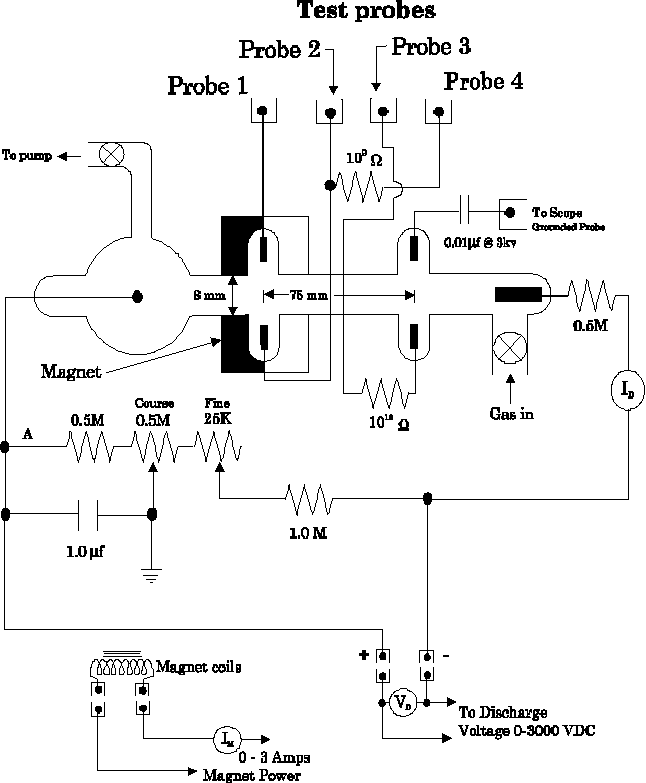
\includegraphics[width=0.45\textwidth]{plots/apparatus.png}
\caption{Experimental setup. Probe 1-2 measures the Hall Voltage ($V_H$) and Probe 2-3 measures the discharge voltage applied to the gas.}
\label{setup}
\end{figure}
\paragraph{Instrumentation} 
\paragraph{Procedures}

\section{Analysis}\label{sec:analysis}
%Analysis:  the calculations that the lab manual asks you to do are supposed to act as a guide to your analysis, and not as a series of separate calculations. agree with prediction? error analysis? source of error, uncertainty?  
The discharge voltage has an approximately linear relationship with the discharge current.
\subsection{Magnetic field as a function of current}
Since the magnetic field in this experiment is provided by a Helmholtz coil, there may be hysteresis behavior due to the ferromagnetic nature of the materials \cite{3_sethna_1994}. So we measure the magnetic field as a function of current for various gas pressures to make sure that hysteresis is not a huge effect.  It is important to distinguish between the magnetic current $I_m$  that we measure in this experiment with the direct current supplied to the Helmholtz coil $I_d$. By doing linear regression, we can see that the combination of forward/reverse polarity and increasing/decreasing current in the hysteresis loop seems to conform to a linear relationship. Therefore, we conclude that the non-linearity introduced by the hysteresis effect is not significant to our experiment.
\begin{figure}[h]
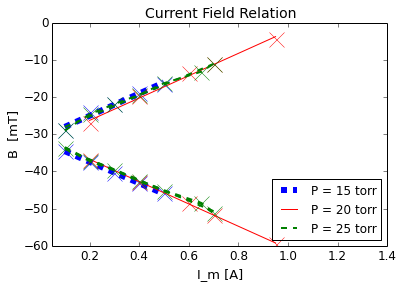
\includegraphics[width=0.45\textwidth]{plots/bim.png}
\caption{Plot of magnetic field strength as a function of magnetic current for three different pressures. The y-intercept approximately correspond to the Earth's magnetic field, since the "zero"-ing function on our magnetometer seems to be malfunctioned.}
\label{bim}
\end{figure}
\begin{table}[]
\centering
\caption{Table of linear regression coefficient (y=mx+b) where (m,b) are the coefficients for the forward polarity and (m',b') for the reverse polarity.}
\label{tbl}
\begin{tabular}{|l|l|l|l|}
\hline
P {[}torr{]} & 15     & 20     & 25     \\ \hline
m            & 29.90  & 30.02  & 28.23  \\ \hline
b            & -31.03 & -32.29 & -30.86 \\ \hline
m'           & -28.70 & -30.00 & -27.85 \\ \hline
b'           & -31.69 & -30.74 & -31.19 \\ \hline
\end{tabular}\end{table}
\subsection{Magnetic Field as a function of Hall Voltage}
We measured the Hall Voltage ($V_H$) by varying the magnetic field and conducted this experiment at three different pressures. The Hall field is related to the Hall Voltage that we measure by Eq. \ref{hall_field}. As we expect, the relationship between Hall Voltage and magnetic field is approximately linear, with the exception of P=15 torr dataset, which was affected significantly by non-linearity and oscillations.  The fitting coefficients are described in Table. \ref{fit} Using Eq.\ref{EHBV},\ref{hall_field}, we can obtain a linear relationship between $V_H$ and B, assuming that electrons are travelling perpendicular to the direction of B: 
\begin{equation}
V_H = (4mm v)B
\label{BV}
\end{equation}
\begin{table}[]
\centering
\caption{The linear regression coefficients for the hall voltage v.s. magnetic field relationship. Note that the P=15 torr dataset was measured when there was oscillations and striation in the plasma. Therefore there was a significant amount of nonlinearity in the B-$V_H$ relationship, which suggests that the m,b values for P=15 torr is not a very accurate summary of the data.}
\label{fit}
\begin{tabular}{|l|l|l|l|}
\hline
P {[}torr{]} & 15     & 20     & 25    \\ \hline
m            & -1.64  & -3.70  & -0.31 \\ \hline
b            & -31.21 & -31.66 & -9.45 \\ \hline
\end{tabular}
\end{table}
We show the linear plots for the magnetic field measured with the forward and reverse polarities combined. The non-zero value of the intercept compared to Eq. \ref{BV} results from the fact that measurements of the potential is relative.

\begin{figure}[h]
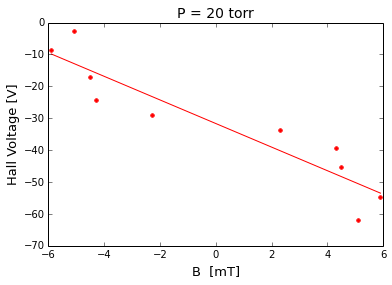
\includegraphics[width=0.40\textwidth]{plots/P20HB.png}
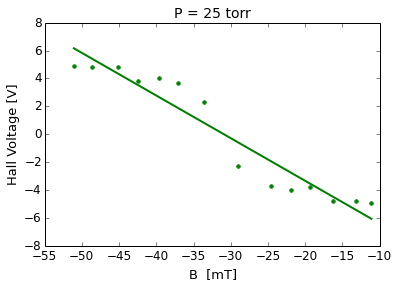
\includegraphics[width=0.40\textwidth]{plots/P25HB.png}
\caption{Plot of Hall Voltage versus Magnetic Field at P = 20 and 25 torr with the forward and reverse polarities combined. The Hall voltage of the reverse field is flipped to a positive sign.}
\label{HBplot}
\end{figure}
\subsection{Plasma Parameters}
Using the relations derived in Sec. \label{sec:plasma_param_theory}, we are able to compute the plasma parameters (v, $n_e$, $\nu$, $<\sigma v>$,$v_{rms}$, $<v>$, $T_e$)
based on the experimental parameters P, B, $I_D$ and  the experimental measurements of  $V_D$, $V_H$. 
The plasma parameters that we obtained are summarized in Table. \ref{pparam}




\begin{table}[]
\centering
\caption{The--- of three selected datasets.}
\label{my-label}
\begin{tabular}{|l|l|l|l|}
\hline
P {[}torr{]}    & 25                 & 20                 & 15                   \\ \hline
I\_D{[}mA{]}    & 0.57$\pm$0.02      & 0.9$\pm$0.02       & 1.61$\pm$0.02        \\ \hline
B {[}mT{]}      & -16.3$\pm$0.1      & -28.9$\pm$0.1      & -21.8$\pm$0.1        \\ \hline
V\_H {[}V{]}    & -4.8$\pm$0.2       & -2.3$\pm$0.2       & -4.8$\pm$0.2         \\ \hline
V\_D{[}V{]}     & -62$\pm$0.2        & -52$\pm$0.2        & -39$\pm$0.2          \\ \hline
$n_e [m^{-3}]$  & $9.6\times10^{14}$ & $5.6\times10^{15}$ & $3.63\times 10^{15}$ \\ \hline
$\nu [s^{-1}]$  & $1.97\times10^9$   & $5.89\times10^9$   & $1.66\times10^9$     \\ \hline
$v_{rms} [m/s]$ & $7.81\times10^5$   & $2.86\times10^5$   & $2.61\times10^5$     \\ \hline
$T_e [K]$       & 21100              & 16300              & 13400                \\ \hline
\end{tabular}
\end{table}
\section{Conclusion}\label{sec:conclusion}
%findings, future improvement? 


\section*{Acknowledgments}
I am sincerely thankful for support from Professor Harmut Haeffner, Kam-Biu Luk, Don Orlando, and my lab partner Xiyue Wang for contributing to successful completion of this lab.
\bibliographystyle{SIGCHI-Reference-Format}
\bibliography{sample}

%Raw Data: You must include the data that you took in lab in an appendix; the data should be clear enough so that someone could look at it and determine what you measured and how you measured it. You should be keeping a lab notebook, so simply photocopy all relevant pages. Your report should include all of the listed sections, along with the signed Pre-lab and Mid–Lab Discussion sheets.

\end{document}


